\documentclass{beamer}
\usepackage{color}
\usepackage{xcolor}
\usepackage[backend=biber]{biblatex}
\usepackage{tikz}
\usepackage{amssymb}
\usepackage[toc]{multitoc}
\usepackage{wrapfig}
\usepackage{subfig}
\usepackage{graphicx}
\usepackage{mathrsfs}
\usepackage{animate}

\renewcommand*{\multicolumntoc}{2}
\setlength{\columnseprule}{1pt}

\setbeamertemplate{bibliography item}{\insertbiblabel}

\RequirePackage{currfile} 
\setbeamertemplate{caption}[numbered]

\usetheme{Frankfurt}
%\usecolortheme{whale}

\addbibresource{main.bib}



%\logo{
\includegraphics[width = 0.5 in]{Figures/epscor.jpeg}}

\definecolor{maincol}{HTML}{4B778D}
\definecolor{secondcol}{RGB}{75,119,141}
\definecolor{thirdcol}{RGB}{40,181,181}
\definecolor{orangeCoral}{HTML}{FFC996}
\definecolor{turfGreen}{HTML}{BDD2B6}
\definecolor{algaeRed}{HTML}{CF0000}
\definecolor{parrotBlue}{HTML}{4974A5}
\setbeamercolor{palette primary}{bg = maincol, fg=white}
\setbeamercolor{palette secondary}{bg = secondcol, fg=white}
\setbeamercolor{palette tertiary}{bg=thirdcol, fg=white}
\setbeamercolor{palette quaternary}{bg = thirdcol, fg=white}
\setbeamercolor{structure}{fg=maincol}
\setbeamercolor{section in toc}{fg=maincol} 
\setbeamercolor{subsection in head/foot}{bg=maincol, fg=white}

%--------Stuff for Compartment/Blocks-----%
\usetikzlibrary{arrows}
\tikzstyle{block} = [rectangle, draw, fill=orangeCoral, text width = 1.5em, text centered, minimum height = 2em]
\tikzstyle{blockTurf} = [rectangle, draw, fill=turfGreen!50, text width = 1.5em, text centered, minimum height = 2em]
\tikzstyle{blockAlgae} = [rectangle, draw, fill=algaeRed!45, text width = 1.5em, text centered, minimum height = 2em]
\tikzstyle{blockParrot} = [rectangle, draw, fill=parrotBlue!50, text width = 1.5em, text centered, minimum height = 2em]
\tikzstyle{line} = [thick, ->, >= stealth]
\tikzstyle{noblock} = [rectangle, draw = none]

%%--------------- Title Slide ------------------------------
\title[]{Effects of Overfishing on Coral Reef Ecosystems}
\subtitle{Coral Reefsearchers}
\author{Aaron Bumagat, Michelle Luces, Henry Song }
\institute{University of Guam}
\date{\today} 


\begin{document}
\frame{\titlepage}

\AtBeginSection[]{
    \begin{frame}{}
        \frametitle{}
        \setcounter{tocdepth}{2}
        \tableofcontents[currentsection, sections = \thesection]
        \setcounter{tocdepth}{1}
    \end{frame}
}
% \AtBeginSection[]{}
% \begin{frame}<Beamer>
% \frametitle{}
% \setcounter{tocdepth}{2}
% \tableofcontents{currentsection, sections = \thesection}
% \setcounter{tocdepth}{1}
% \end{frame}

%%------------------Table of Contents---------------------------
\begin{frame}{Table of Contents}
    \tableofcontents
\end{frame}

%%-----------------------Introduction-------------------------

%%--------------------------Background--------------------------
\section{Background}
% \begin{frame}{Background}
%     \begin{itemize}
%         \item Coral Reefs are large underwater structures composed of the skeletons of colonial marine invertebrates known as coral$^\cite{ross}$.
%     \end{itemize}
% \end{frame}
% \begin{frame}{Background}
%     \begin{itemize}
%         \item Coral Reefs are large underwater structures composed of the skeletons of colonial marine invertebrates known as coral$^\cite{ross}$.
%         \item Climate change is a leading factor for the cause of coral bleaching/death.
%     \end{itemize}
% \end{frame}
% \begin{frame}{Background}
%     \begin{itemize}
%         \item Coral Reefs are large underwater structures composed of the skeletons of colonial marine invertebrates known as coral$^\cite{ross}$.
%         \item Climate change is a leading factor for the cause of coral bleaching/death.
%         \item Overfishing, temperature changes, and resiliency of coral reef species are factors when it comes to the changes in a reef ecosystem.
%     \end{itemize}
% \end{frame}

\subsection{General Background}
\begin{frame}{Background}
    \begin{itemize}
        \item<1-> Coral Reefs are large underwater structures composed of the skeletons of colonial marine invertebrates known as coral\textsuperscript{\cite{ross}}.
         \item<2-> They play a crucial role in the marine ecosystem's biodiversity along with other functions, such as coastal defense from storms and economic benefits from tourism or local fisheries\textsuperscript{\cite{04_mathanalysis}}.
         \item<3-> According to the 2008 State of the Coral Reef Ecosystems of Guam report, Guam’s coral reef resources are both economically and culturally important, providing numerous goods and services for the residents of Guam, including cultural/traditional use, tourism, recreation, fisheries, and shoreline/infrastructure protection \textsuperscript{\cite{guamwebsite}}.
         \item<4-> Factors that affect coral reefs include climate change, coral reef resilience\textsuperscript{\cite{02_Riegl_Purkis_Model}}, and exploitative fishing practices\textsuperscript{\cite{05_quintero_machuca_cotto_bradley_ríos-soto_2016}}.
    \end{itemize}
\end{frame}

\subsection{General Question}
\begin{frame}{Our Question}
\begin{itemize}
    \item General Question: How will Guam's reef ecosystem change over the coming decades?
\end{itemize}
\begin{center}
    $\Downarrow$
\end{center}
\begin{itemize}
    \item Specific Question: How will overfishing affect Guam's coral reef ecosystem in the upcoming decades?
\end{itemize}
\begin{figure}
    \centering
    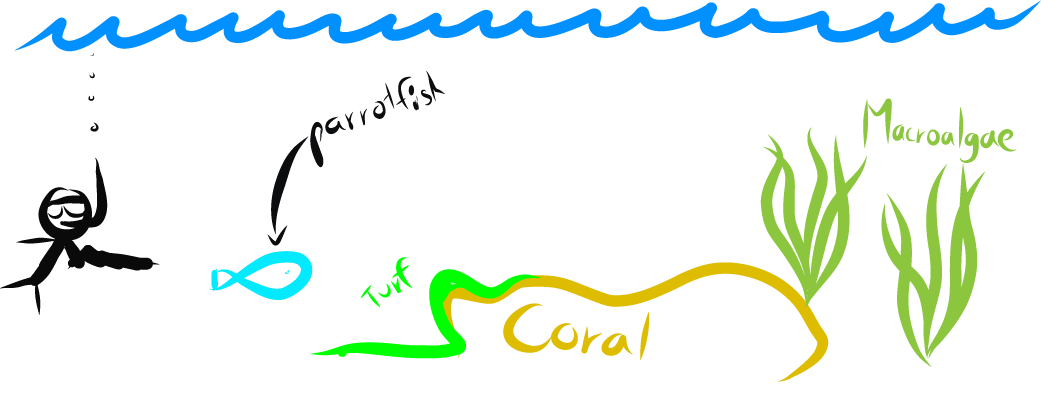
\includegraphics[width=0.9\textwidth]{Latex/Figures/figure1.png}
    %\caption{Caption}
    %\label{fig:my_label}
\end{figure}
\end{frame}

\subsection{Definitions}
\begin{frame}{Identify Our Terms}
    \begin{figure}%
        \centering
        \subfloat[\centering Corals\textsuperscript{\cite{img_coral_reef}}]{{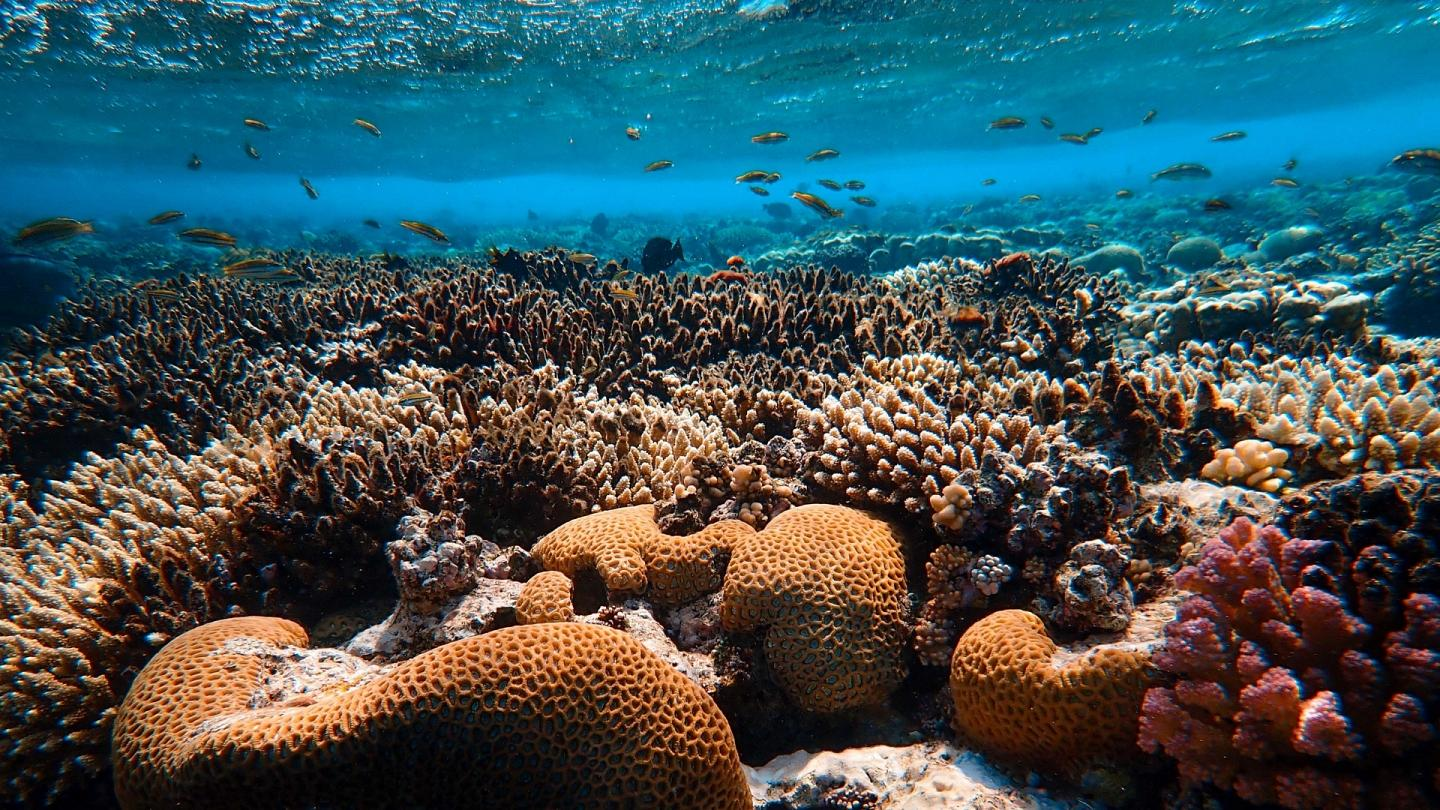
\includegraphics[width=4.7cm]{Latex/Figures/coral_reefs.jpg} }}%
        \\
        \subfloat[\centering Algal Turfs\textsuperscript{\cite{img_algal_turf}}]{{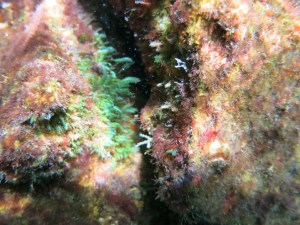
\includegraphics[width=3.5cm]{Latex/Figures/algal_turf.jpg} }}%
        \qquad
        \subfloat[\centering Macroalgae\textsuperscript{\cite{img_macroalgae}}]{{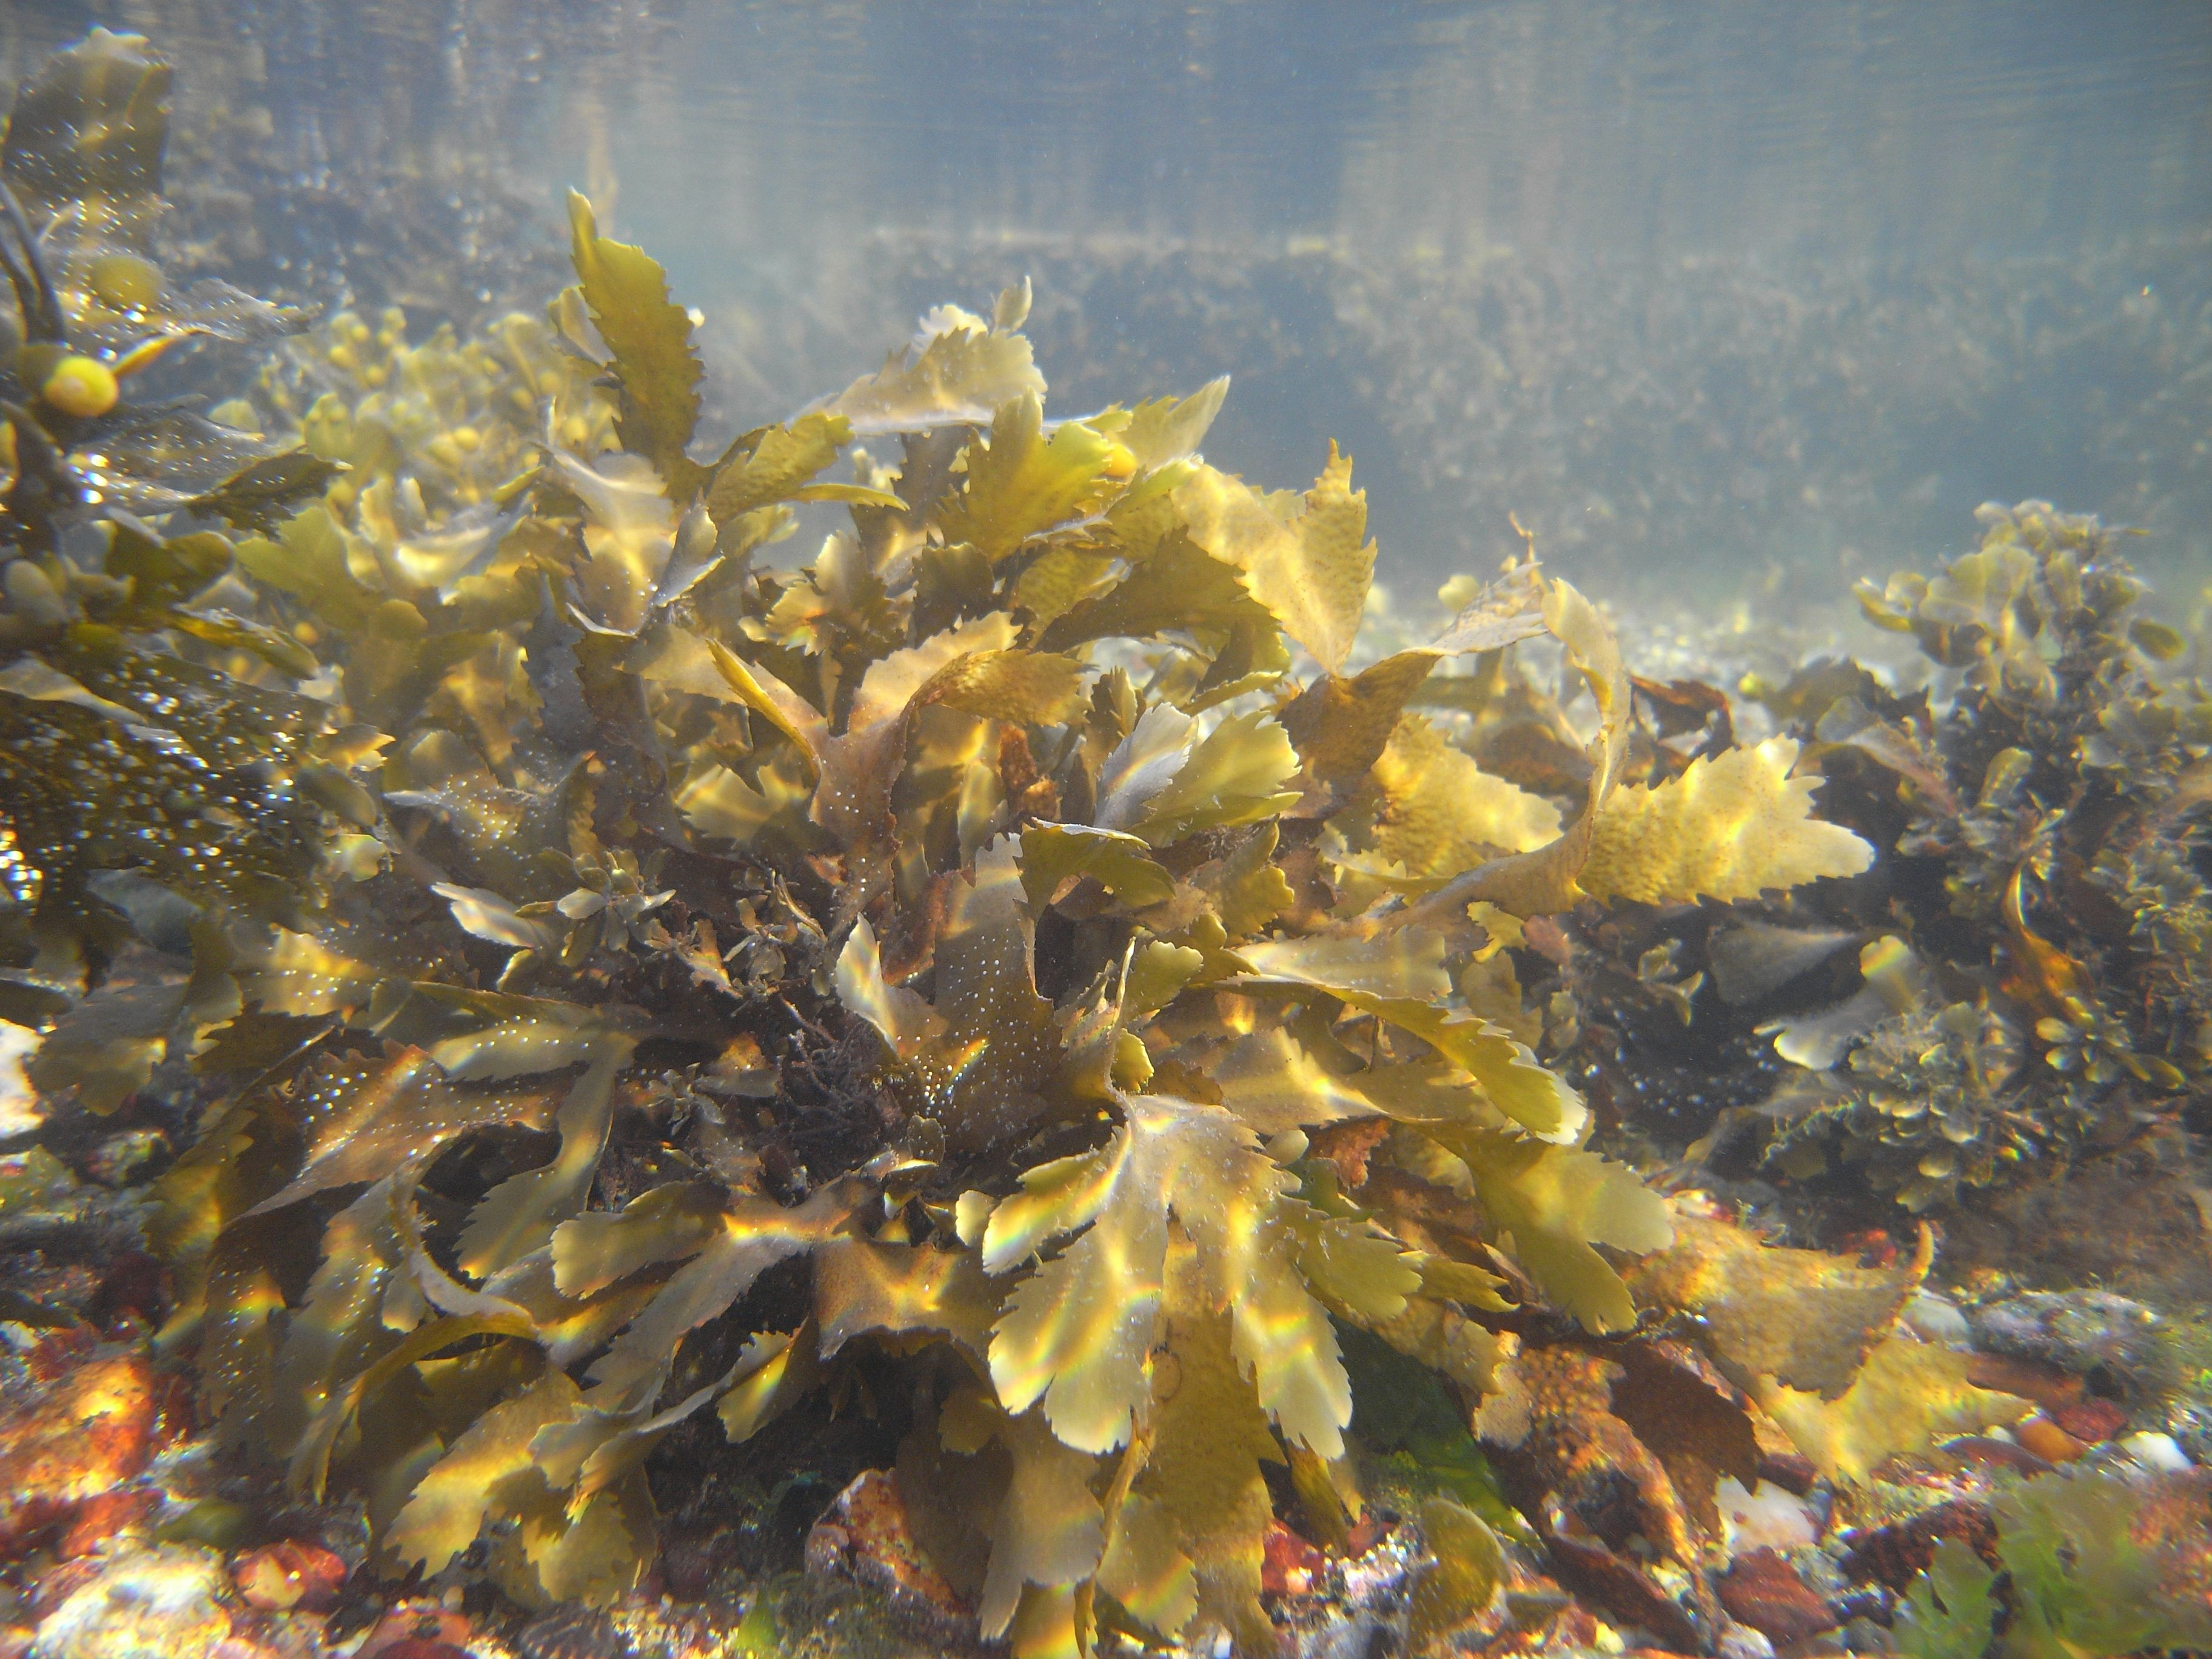
\includegraphics[width=3.5cm]{Latex/Figures/macroalgae.jpg} }}%
        \caption{Images of Ecosystem}%
        \label{fig:graphs}%
    \end{figure}
\end{frame}

\begin{frame}{Identify Our Terms (Cont.)}
    \begin{columns}
        \begin{column}{0.5\textwidth}
            \begin{figure}
                \centering
                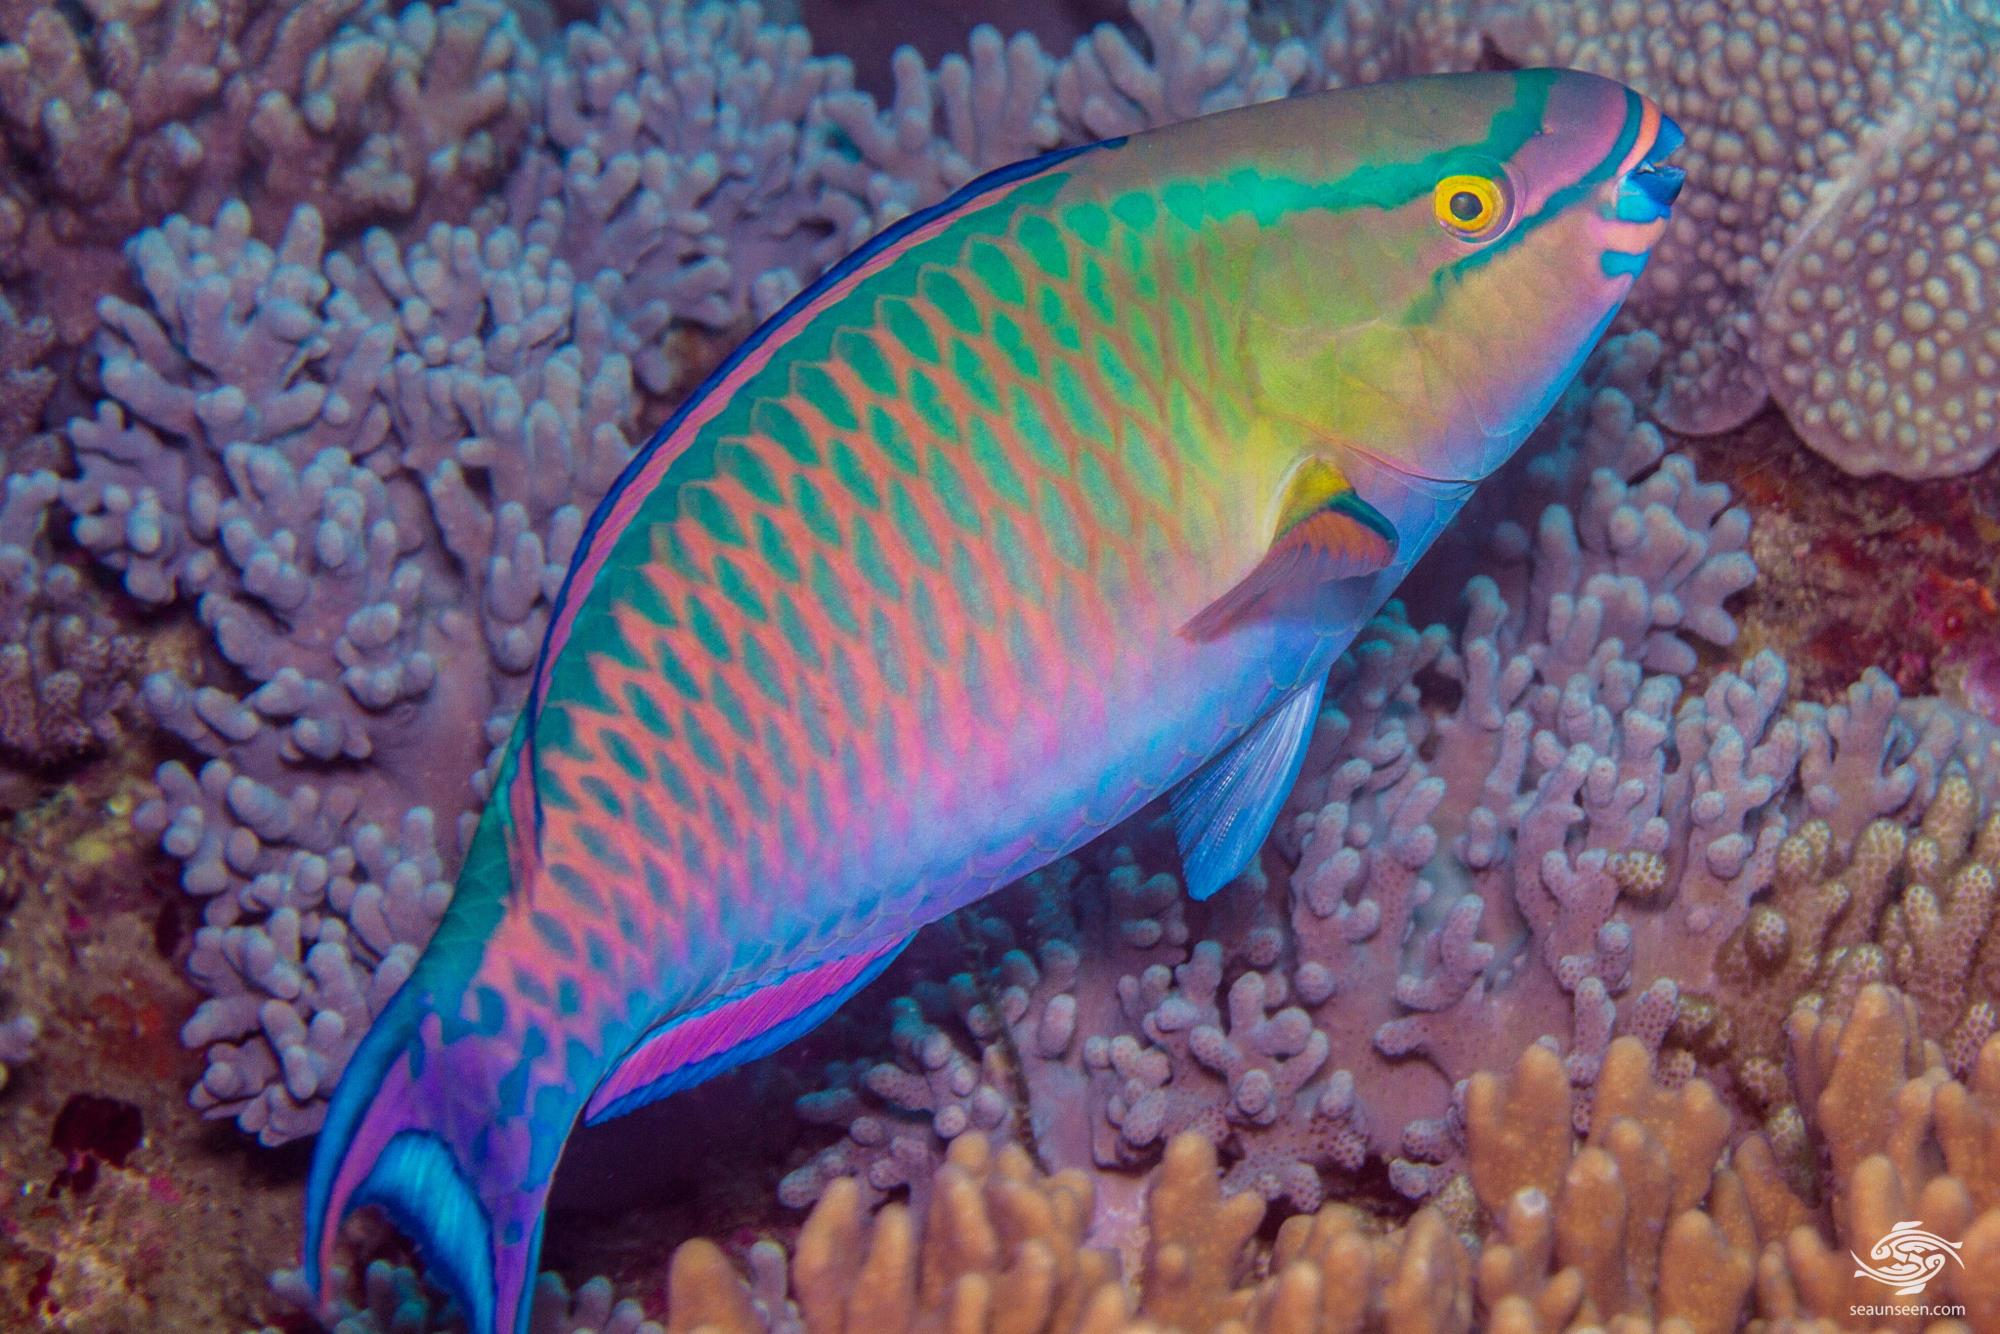
\includegraphics[width=1\textwidth]{Latex/Figures/parrot_fish.jpg}
                \caption{Parrot Fish\textsuperscript{\cite{img_parrot_fish}}}
                \label{fig:my_label}
            \end{figure}
        \end{column}
        \begin{column}{0.5\textwidth}
            \begin{itemize}
                \item Parrot fish are common reef fish found in many tropical reefs\textsuperscript{\cite{13_blackwood_hastings_mumby_2010}} and are known to feed on algal turfs and macroalgae.
                \item Their bites on corals have been shown to improve and promote coral growth.
                \item Parrot fish are one of the most overfished reef fish in the Caribbean, and potentially on Guam as well\textsuperscript{\cite{13_blackwood_hastings_mumby_2010}}.
            \end{itemize}
        \end{column}
    \end{columns}
    % \begin{wrapfig}{l}
    %     \centering
    %     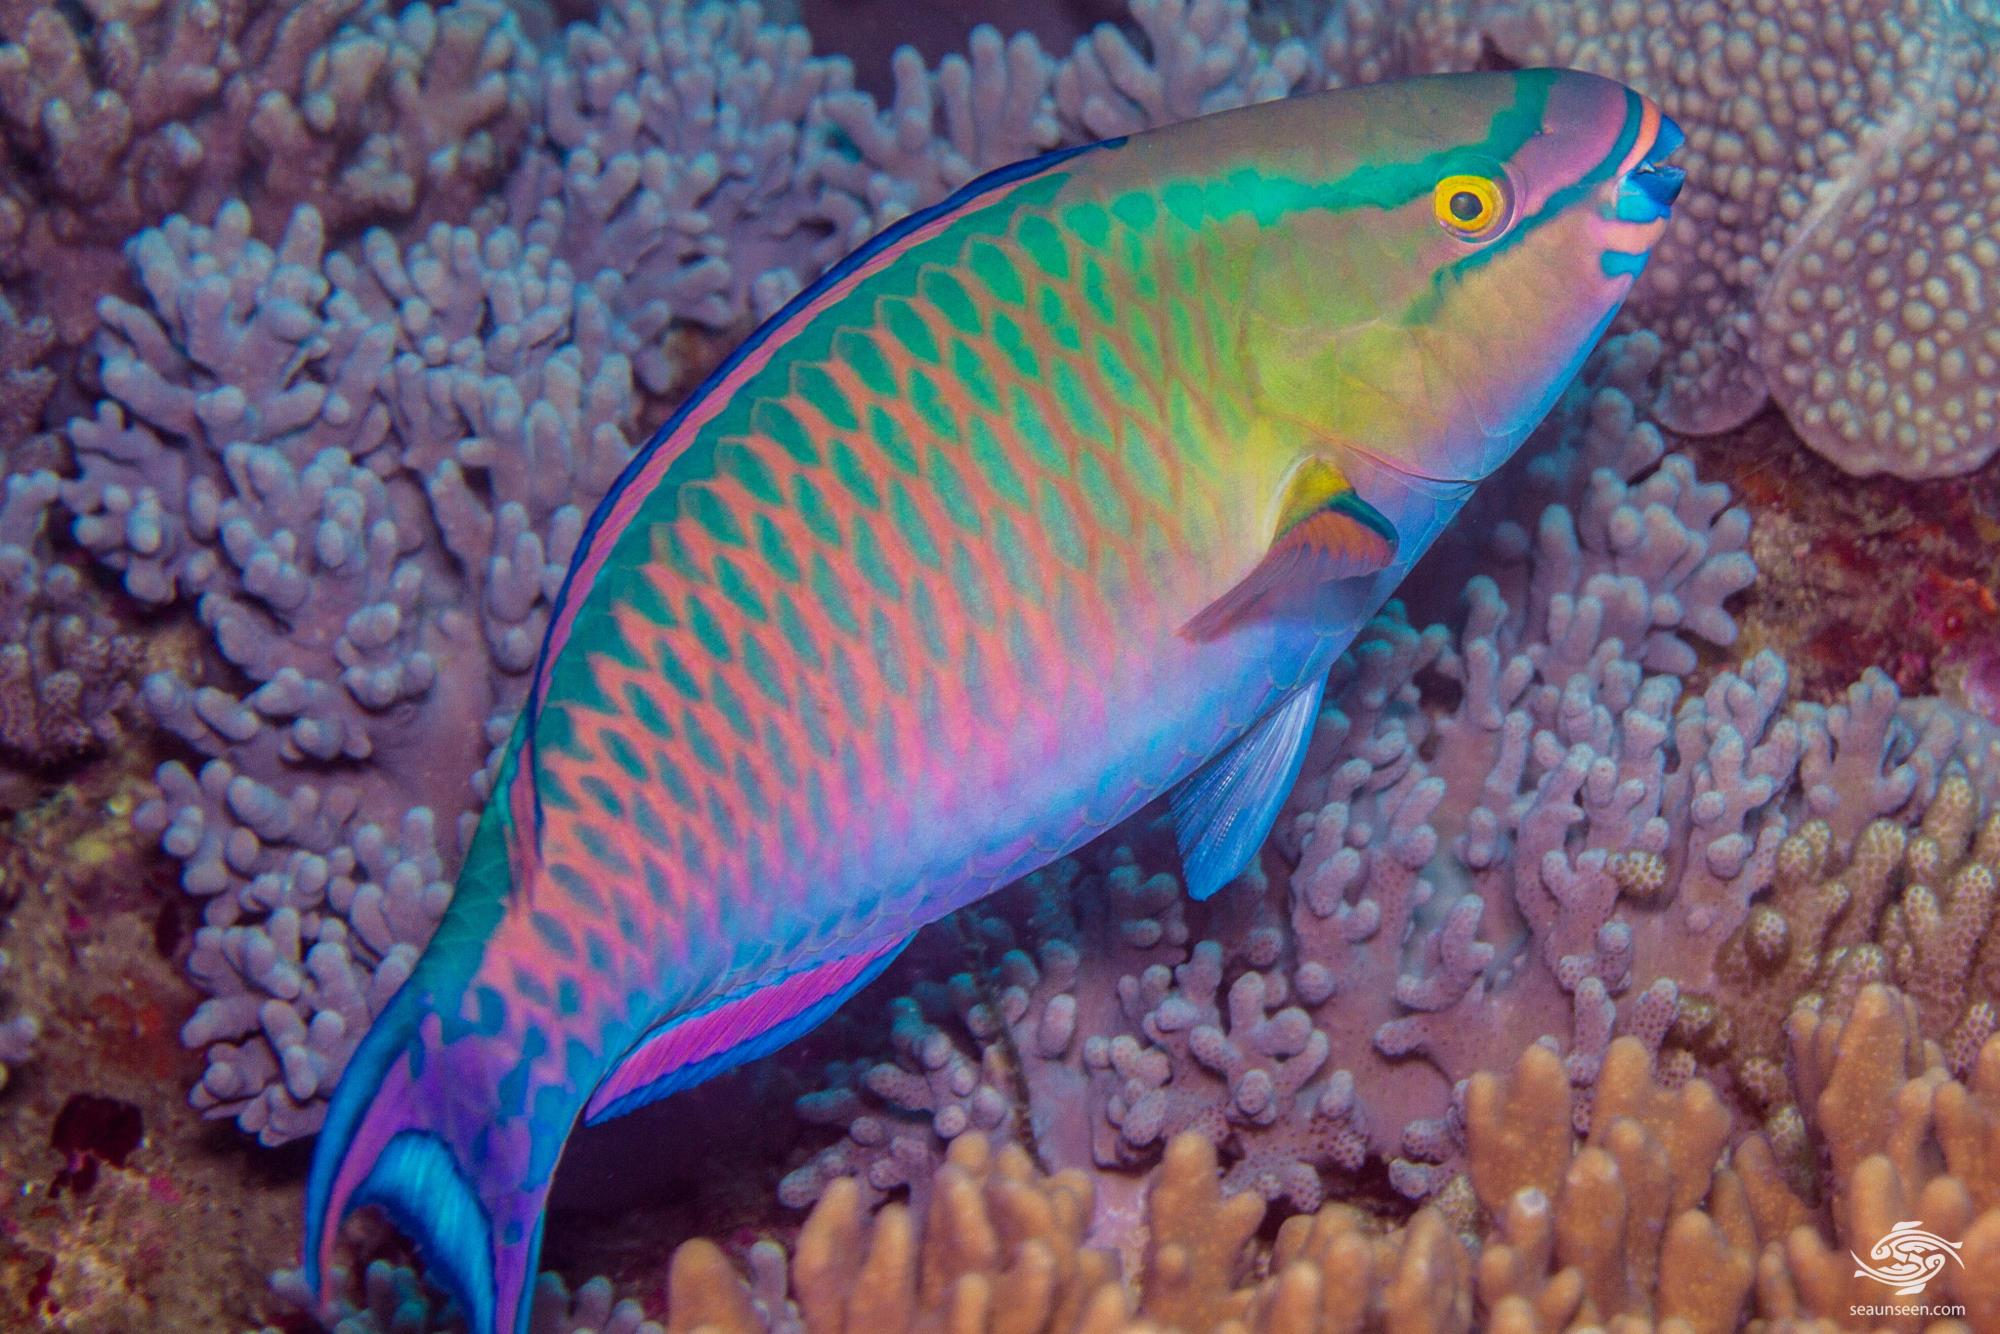
\includegraphics[width=0.45\textwidth]{Latex/Figures/parrot_fish.jpg}
    %     \caption{Parrot Fish\textsuperscript{\cite{img_parrot_fish}}}
    %     \label{fig:my_label}
    % \end{wrapfig}
\end{frame}


%%------------------------Literature Review----------------
%\section{Literature Rev

    %\begin{itemize}
                %\item Can be used to see which will be focused on when creating our parameters.
            %\end{itemize}
    %\end{itemize}
%\end{frame}

%\begin{frame}{Prioritizing Key Resilience Indicators to Support Coral Reef Management in a Changing Climate Cont.}
%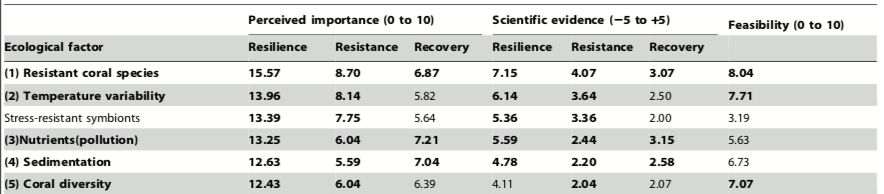
\includegraphics[width = 4.3 in. , height = 1.7 in.]{Figures/Resilience Data.png}
%\end{frame}

%\subsection{Model of coral population response to accelerated bleaching and mass
%mortality in a changing climate}
%\begin{frame}{Model of coral population response to accelerated bleaching and mass mortality in a changing climate}
%    \begin{block}{Summary}
        %Researchers studied coral populations located within the Arabian Peninsula. The study primarily focused on the Porites and %\textit{Acropora} species of coral. The researchers found that coral populations can survive more extreme conditions.
    %\end{block}
%\end{frame}

%\begin{frame}{Model of coral population response to accelerated bleaching and mass
%mortality in a changing climate (Cont.)}
    %Why is this article important?
    %\begin{itemize}
        %\item Methods used include a system of differential equations.
        %\item It implements a compartment model to illustrate the relationships.
        %\item It uses the Lotka-Volterra model to simulate a predator prey relationship between \textit{Acropora} as the dominant species and others as the recessive species.
        %\begin{itemize}
            %\item Incorporates ideas of Game Theory into methods.
        %\end{itemize}
    %\end{itemize}
%\end{frame}

%\subsection{Mathematical Analysis of Coral Reef Models}
%\begin{frame}{Mathematical Analysis of Coral Reef Models}
    %\begin{block}{Summary}
        %This research analyzes grazing in response to threatened coral reef systems. Specifically, this model is focused on the impact of different grazing intensities and their influences on coral-algae interactions. Results provided from this research can provide insight on how to revitalize unhealthy reefs.
    %\end{block}
%\end{frame}

%\begin{frame}{Mathematical Analysis of Coral Reef Models (Cont.)}
    %Why is this article important?
    %\begin{itemize}
        %\item The authors used ordinary differential equations (ODE) and delay differential equations (DDE) to model coral reefs.
        %\item  The mathematical results can help answer how to reverse the unhealthy reefs to a healthy status by knowing how overfishing affects our reefs.
    %\end{itemize}
%\end{frame}

%%------------------------------------------------------


%%-----------------------------Math-------------------------
\section{Mathematical Model} % & Analysis
\subsection{Assumptions}
\begin{frame}{Assumptions}
    \begin{itemize}
        \item Ecosystem:
        \begin{itemize}
            \item is closed (i.e. no migration).
            \item consists of only corals (C), algal turfs (T), and macroalgae (M).
            \item supports maximum carrying capacity of parrotfish.
        \end{itemize}
        \item Macroalgae is the only predator for coral.
        \item Coral recruit to and overgrow algal turfs\textsuperscript{\cite{04_mathanalysis}}.
        \item Corals are overgrown by macroalgae\textsuperscript{\cite{04_mathanalysis}}.
        \item Macroalgae colonize dead coral by spreading vegetative over algal turfs (T)\textsuperscript{\cite{04_mathanalysis}}.
        \item Corals do not naturally die.
        % \item Macroalgae is the only predator for Coral.
        % \item Rates are measured in year(s).
        % \item Coral recruit to and overgrow Algal Turfs\textsuperscript{\cite{04_mathanalysis}}.
        % \item Corals are overgrown by Macroalgae\textsuperscript{\cite{04_mathanalysis}}.
        % \item Macroalgae colonize dead Coral by spreading vegetative over algal turfs\textsuperscript{\cite{04_mathanalysis}}.
        % \item Coral natural death rate is nonexistent (i.e. not from Macroalgae overgrowth).
        % \item Algal turf and macroalgae do not have a death rate.
    \end{itemize}
\end{frame}

\subsection{Compartments}
\begin{frame}{Coral Reef Ecosystem Model Compartments}
    \begin{block}{Compartments}
    The Ecosystem Model consists of 4 compartments:
        \begin{itemize}
        \item \small{$C$: Corals}
        \item \small{$T$: Algal Turfs}
        \item \small{$M$: Macroalgae}
        \item \small{$P$: Parrotfish}
        \end{itemize}
        $$ \text{where } C + T + M = 1.$$
    \end{block}
\end{frame}

\subsection{Parameters}
\begin{frame}{Coral Reef Ecosystem Model Parameters}
    \begin{table}
    %\centering
    \vspace{-.7cm}
    \begin{tabular}{c p{5cm} c c}
        \hline
        Parameter & Description & Rate & Units\textsuperscript{\cite{12_noaa_report}\cite{04_mathanalysis}\cite{13_blackwood_hastings_mumby_2010}}\\
        \hline
        \hline
        $\mu_{1}$ & natural death rate of coral reefs & 0.15\textsuperscript{\cite{16_wolanski_richmond_mccook_2004}} & $year^{-1}$\\ %12
        $\mu_{2}$ & natural death rate of parrotfish & 0.22\textsuperscript{\cite{12_noaa_report}} & $year^{-1}$\\ %8
        $r$ & rate that coral recruit to overgrow algal turfs & 10\textsuperscript{\cite{16_wolanski_richmond_mccook_2004}} & $year^{-1}$\\ %12
        %$g$ & grazing rate that parrotfish graze macroalgae without distinction from algae turfs & $\frac{kg}{yrs}$\\
        $\gamma$ & rate that macroalgae spread vegetative over algal turfs & 0.8\textsuperscript{\cite{11_zikkah_anggriani_supriatna_2020}} & $year^{-1}$\\ %13
        $q$ & intrinsic growth rate for parrotfish & 0.47\textsuperscript{\cite{12_noaa_report}} & $year^{-1}$\\ %8
        $h$ & harvesting rate for parrotfish & 0.14\textsuperscript{\cite{12_noaa_report}} & $year^{-1}$\\ %8
        $\sigma$ & rate that parrot fish bite coral & 0.01*& $bites*year^{-1}$\\
        $\alpha$ & maximum grazing intensity & 1* & -\\
        $\beta$ & carrying capacity of parrotfish & 1* & -\\
        $a_{0}$ & control variable to simulate seasonal changes & 0.99 & - %13
    \end{tabular}
    %\caption{Model Parameters}
    %\label{tab:my_label}
\end{table}
* = \textit{estimated value}
\end{frame}

\subsection{Compartment Model}
\begin{frame}{Coral Reef Ecosystem Model\textsuperscript{\cite{04_mathanalysis}}}
\begin{center}
    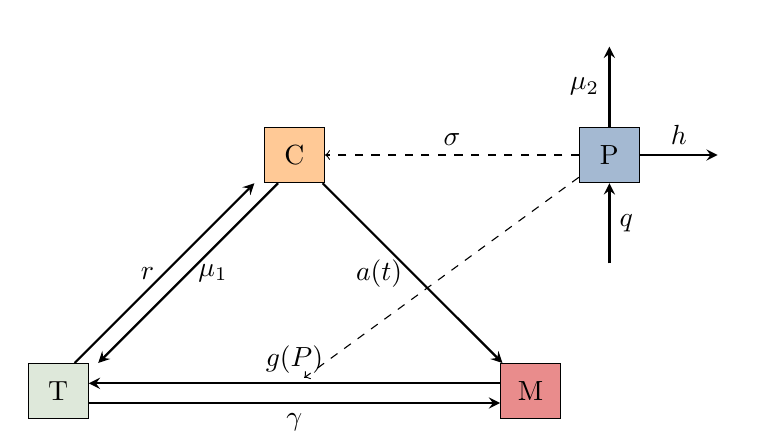
\begin{tikzpicture}{node distance = 1cm, auto}
        \node(leftofC) [noblock] {}; 
        \node(C) [block, right of = leftofC, node distance = 1.5 cm] {C};
        \node(P) [blockParrot, right of = C, node distance = 4 cm] {P};
        \node(belowofC) [noblock, below of = C, node distance = 3 cm]{};
        \node(M) [blockAlgae, right of = belowofC, node distance = 3 cm] {M};
        \node(T) [blockTurf, left of = belowofC, node distance = 3 cm] {T};
        \node(rightofP) [noblock, right of = P, node distance = 1.5 cm]{};
        \node(aboveofP) [noblock, above of = P, node distance = 1.5 cm]{};
        \node(aboveofC) [noblock, above of = C, node distance = 1.5 cm]{};
        \node(belowofP) [noblock, below of = P, node distance = 1.5 cm]{};
        \node(aboveofT) [noblock, above of = T, node distance = 0.08 cm]{};
        \node(diagonalofT) [noblock, right of = aboveofT, node distance = 3 cm]{};
        \draw[dashed, ->] (P) --node[above]{} (diagonalofT);
        \draw[dashed, ->] (P) --node[above]{$\sigma$} (C);
        \draw[line] (C) --node[left]{$a(t)$} (M);
        \draw[line] (P) --node[above]{$h$} (rightofP);
        \draw[line] (P) --node[left]{$\mu_{2}$} (aboveofP);
        %\draw[line] (C) --node[left]{$d$} (aboveofC);
        \draw[line] (belowofP) --node[right]{$q$} (P);
        \begin{scope}[transform canvas = {xshift = -.15cm}]
            \draw[line](T) -- node[left]{$r$} (C);
        \end{scope}
        \begin{scope}[transform canvas = {xshift = .15cm}]
            \draw[line](C) --node[right]{$\mu_{1}$} (T);     
        \end{scope}
        \begin{scope}[transform canvas = {yshift = .1cm}]
            \draw[line] (M) --node[above]{$g(P)$} (T);
        \end{scope}
        \begin{scope}[transform canvas = {yshift = -.15cm}]
            \draw[line] (T) --node[below]{$\gamma$} (M);
        \end{scope}
    \end{tikzpicture}
\end{center}
\end{frame}

\subsection{Equations}
\begin{frame}{Differential Equations}
    System of differential equations derived from compartment model:
    \begin{align*}
        \begin{split}
            \frac{dC}{dt} &= rTC + \sigma PC- (a(t)M+\mu_{1})C\\
            \frac{dP}{dt} &= qP \left( 1-\frac{P}{\beta C} \right) - P \left( h+\mu_{2} \right)\\
            \frac{dT}{dt} &= \mu_{1}C + \frac{g(P)M}{M+T} - T(rC+\gamma M)\\
            \frac{dM}{dt} &= (a(t)C+ \gamma T)M - \frac{g(P)M}{M+T}
            \label{SoODE}
        \end{split}
    \end{align*}
    where $g(P) = \frac{\alpha P}{\beta}, \quad a(t)=|\frac{a_{0}(9\sin{(\pi x) }+1)}{10}|$.\\ 
    \quad
    \begin{center}
        \textit{Modified from Blackwood Paper\textsuperscript{\cite{13_blackwood_hastings_mumby_2010}}}
    \end{center}
\end{frame}

\begin{frame}{Simulating $a$}
    \includegraphics[]{Latex/Figures/sin_graph_animation.gif}
\end{frame}

\subsection{Plots}
\begin{frame}{Coral Ecosystem Model Dynamics}
    \begin{figure}
        \centering
        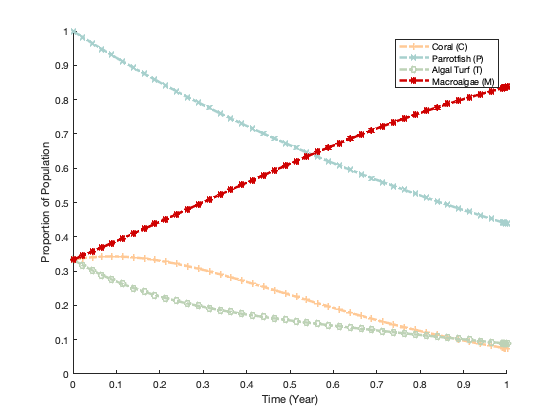
\includegraphics[width=0.9\textwidth]{Latex/Figures/initial_matlab_plot.png}
        \caption{Initial Conditions: $C = T = M = \frac{1}{3}$, and $P = 1$}
        \label{fig:initial_plot}
    \end{figure}
\end{frame}

\begin{frame}{Coral Ecosystem Model Dynamics (Cont.)}
    \begin{figure}
        \centering
        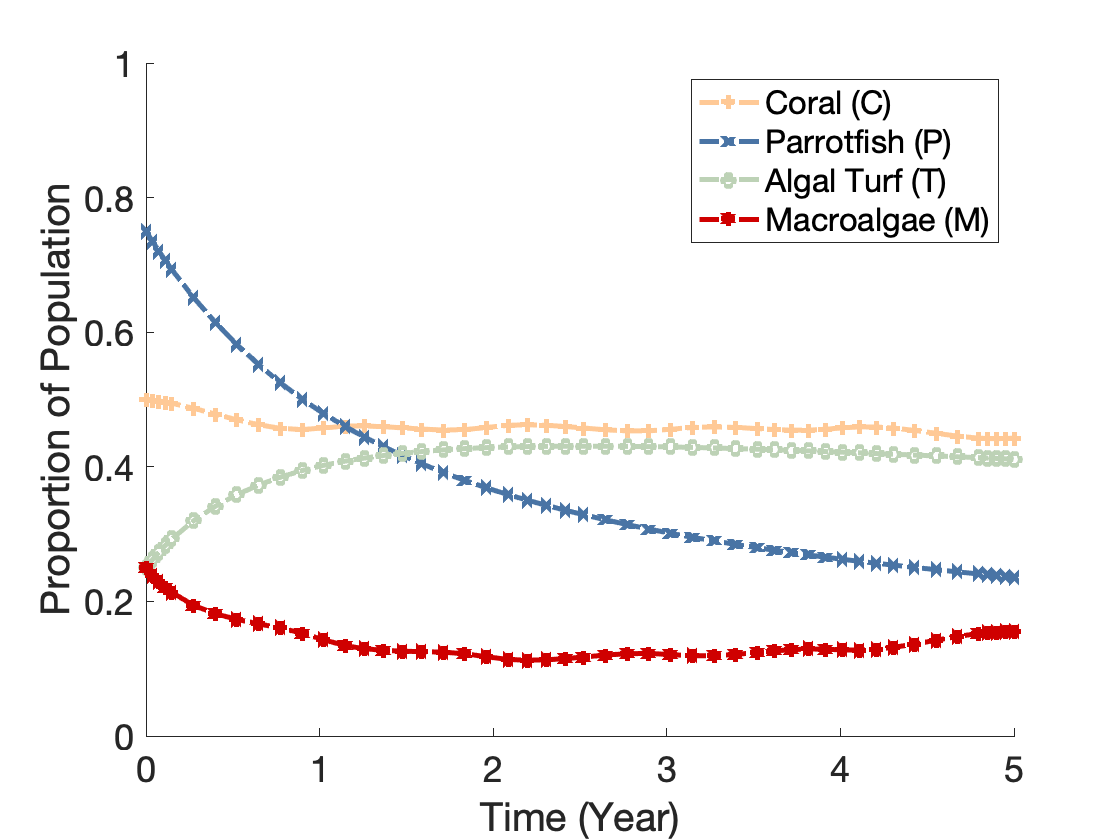
\includegraphics[width=0.9\textwidth]{Latex/Figures/0.5C_0.25T_0.25M.png}
        \caption{Initial Conditions: $C = \frac{1}{2}$, $T = M = \frac{1}{4}$, and $P = 1$}
        \label{fig:coral_dominant}
    \end{figure}
\end{frame}

\begin{frame}{Coral Ecosystem Model Dynamics (Cont.)}
    \begin{figure}
        \centering
        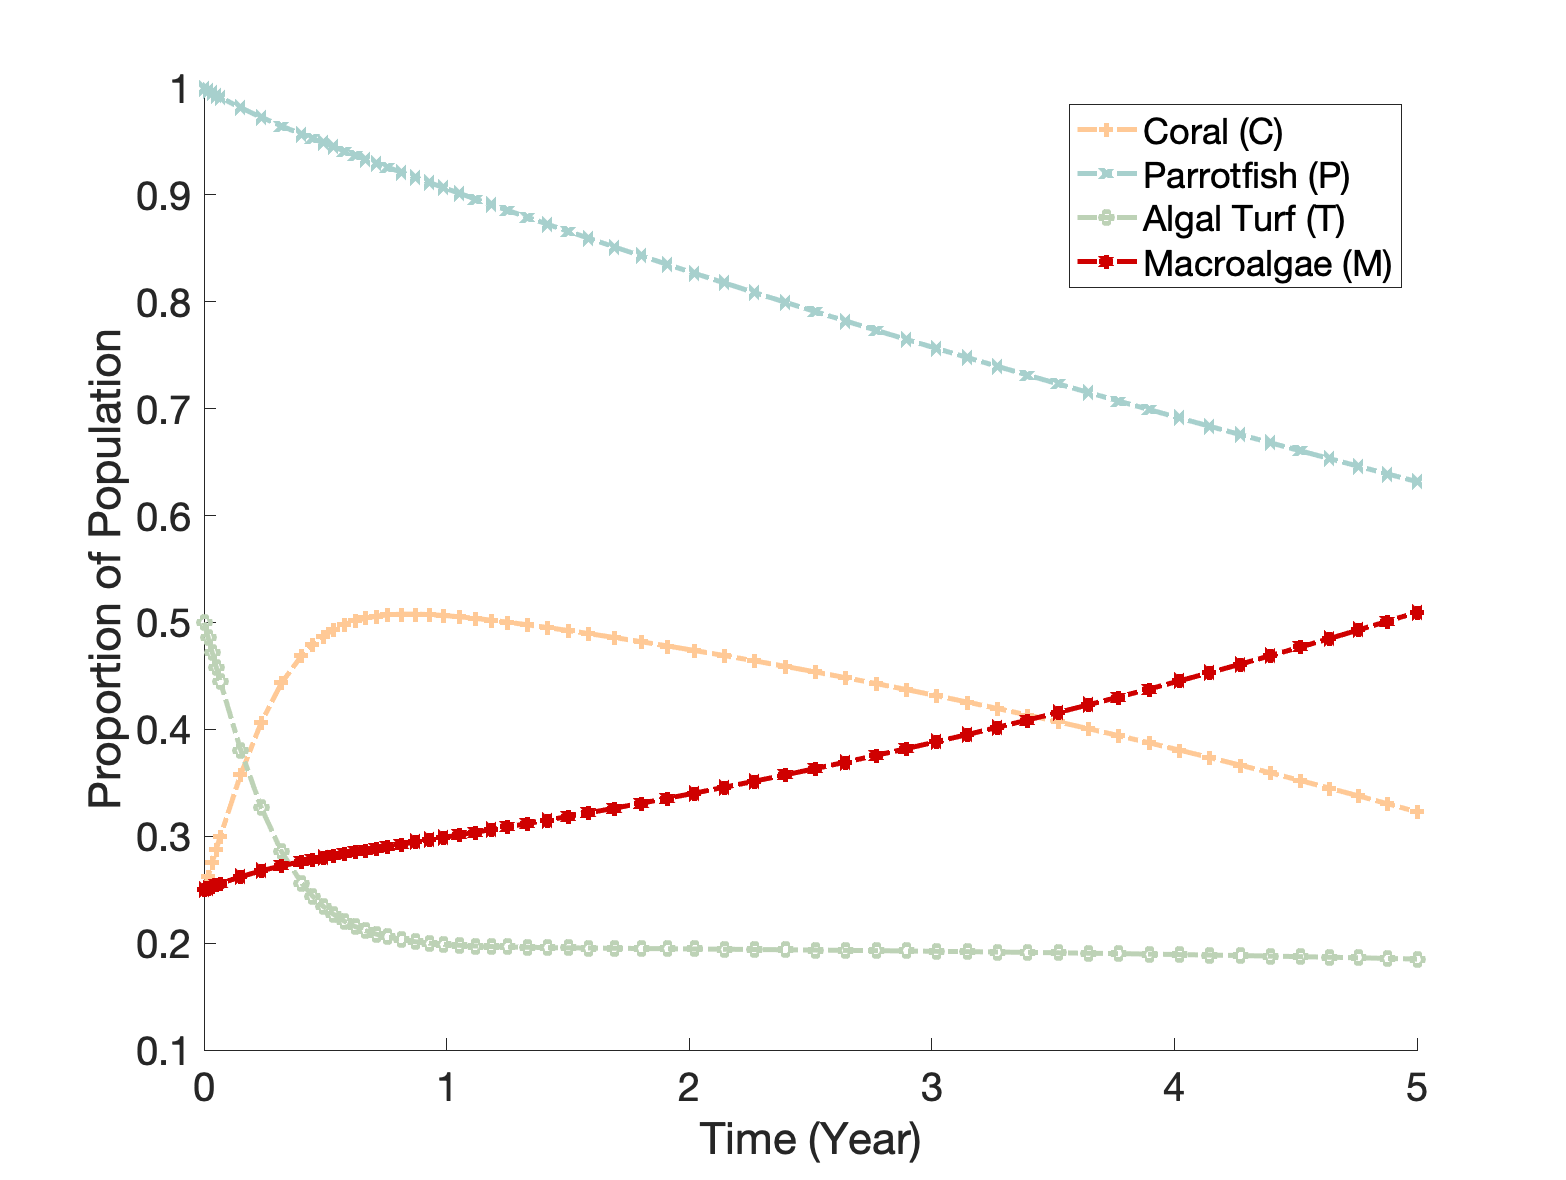
\includegraphics[width=0.85\textwidth]{Latex/Figures/0.25C_0.5T_0.25M.png}
        \caption{Initial Conditions: $T = \frac{1}{2}$, $C = M = \frac{1}{4}$, and $P = 1$}
        \label{fig:turf_dominant}
    \end{figure}
\end{frame}

\begin{frame}{Coral Ecosystem Model Dynamics (Cont.)}
    \begin{figure}
        \centering
        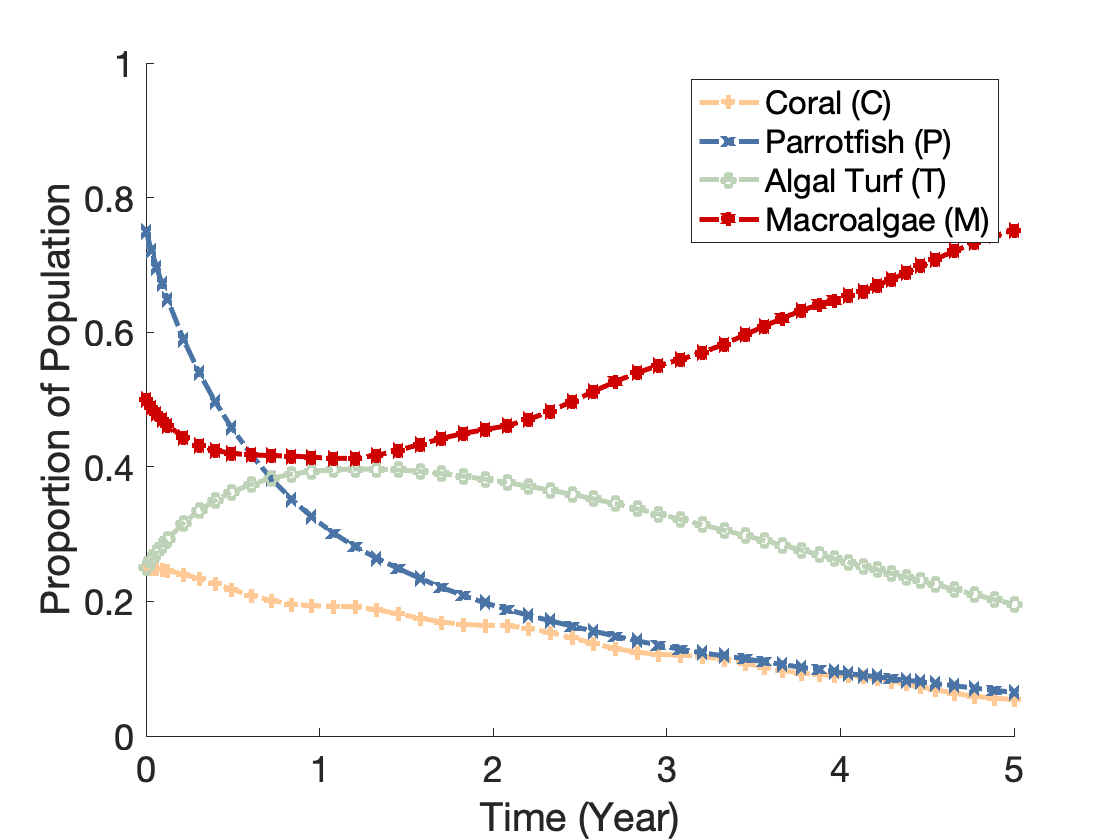
\includegraphics[width=0.9\textwidth]{Latex/Figures/0.25C_0.25T_0.5M.png}
        \caption{Initial Conditions: $M = \frac{1}{2}$, $C = T = \frac{1}{4}$, and $P = 1$}
        \label{fig:macroalgae_dominant}
    \end{figure}
\end{frame}

\subsection{Disease Free Equilibrium (DFE)}
\begin{frame}{Disease Free Equilibrium}
    \begin{align*}
        C^{0} &= 1 - \frac{\mu_{1}}{r}\\
        P^{0} &= -\frac{\beta(1 - \frac{\mu_{1}}{r})(h - \mu_{2} - q)}{q}\\
        T^{0} &= \frac{\mu_{1}}{r}\\
        M^{0} &= 0 \Longleftarrow \text{our "disease" compartment}
    \end{align*}
    \begin{block}{Note}
    Since C + T + M = 1, if $M^{0} = 0$, then $C^{0} + T^{0} = 1$.
    \end{block}
\end{frame}

\subsection{Endemic Equilibrium}
\begin{frame}{Endemic Equilibrium}
    \begin{align*}
        C^{*} &= call you back on this lol\\
        P^{*} &= \\
        T^{*} &= \\
        M^{*} &= 
    \end{align*}
\end{frame}

\subsection{Basic Reproduction Number}
\begin{frame}{Basic Reproduction Number = $\mathscr{R}_{0}$}
    $$\mathscr{F} = \begin{bmatrix} aCM+\gamma,TM \end{bmatrix} \quad \quad \mathscr{V} = \begin{bmatrix} \frac{g(P)M}{M+T} \end{bmatrix}$$
    $$\Downarrow \quad \quad \quad \quad \quad \quad \Downarrow$$
    $$F = \begin{bmatrix} 4x54 \end{bmatrix} \quad V = \begin{bmatrix} 4x54 \end{bmatrix}$$
    $$\displaystyle {\mathscr{R}}_{0} = \frac{\mu_{1}(a r - a\mu_{1} + \gamma \mu_{1})}{r^{2}g(P)}$$
\end{frame}

%----------------------------------------------------


%---------------------Plans---------------------
\section{Plans}
\begin{frame}{Future Plans}
    \begin{itemize}
        %\item Specific ideas:
        %\begin{itemize}
           % \item How will a specific coral species change throughout the upcoming decades on Guam?
            %\item Select a representative species of average resiliency (specifically on Guam) and examine how it will change over time through climate changes.
        %\end{itemize}
        %\item Continue to digest articles and literature relevant to our research.
        \item Finish endemic equilibrium calculations.
        \item Perform sensitivity analysis on parameters.
        \item Refine and improve differential equations to improve dynamics
        % analyze diff eqs
        \item Application of Education Game Theory on the harvest rate parameter ($h$) to quantify human behavior and the best strategy to protect coral reef sustainability. These tasks include:
        \begin{itemize}
            \item Payoff Matrix
            \item Dominant and/or mixed equilibrium equations
            \item Nash Equilibrium/Evolutionarily Stable Strategy
            \item Replicator Equation
        \end{itemize}
    \end{itemize}
\end{frame}

%----------------------------------------------------


%---------------------Conclusion---------------------
%\section{Conclusion}
%\begin{frame}{Conclusion}
    %Type conclusion here
%\end{frame}

\section*{Q \& A}
\begin{frame}
    \Huge{Questions?}
\end{frame}

%%-------------------------Acknowledgements----------------
\section*{Acknowledgements}
\begin{frame}{Acknowledgements}
    \begin{center}
        Support for the Young Scholars Research Experience in Mathematics (YSREM)  is through the MAA Tensor SUMMA Program. Support for the MAA National Research Experience for Undergraduates Program (NREUP) is provided by the National Science Foundation (Grant Number DMS-1950644). Support for the NSF EPSCoR project, Guam Ecosystems Collaboratorium for Corals and Oceans (GECCO) is provided by the National Science Foundation (Grant Number DMS-1946352). \\
    \vspace{.2cm}
    \small{Special thanks to the UOG Marine Laboratory(Dr. Bastian Bentlage and Ms. Grace McDermott), our faculty mentors (Dr. JaeYong Choi, Dr. HyunJu Oh, \& Dr. Leslie Aquino), and our Research Assistants (Jaron Bautista \& Regina-Mae Dominguez).}
    
    \begin{figure}
        
\includegraphics[width = 0.20\textwidth]{Figures/MAA_logo_PMS286.jpg}
        \label{MAA}
        
\includegraphics[width = 0.12\textwidth]{Figures/NSF_4-Color_bitmap_Logo.png}
        \label{NSF}
        % 
\includegraphics[width = 0.20\textwidth]{Figures/GECCO.png}
        % \label{gecco}
        
\includegraphics[width = 0.12\textwidth]{Figures/epscor.jpeg}
        \label{epscor}
        
\includegraphics[width = 0.20\textwidth]{Figures/UOG-horizontal.png}
        \label{uog}
    \end{figure}
    \end{center}
\end{frame}




%%----------------------Bibliography-------------------
\section{Bibliography}
\begin{frame}[allowframebreaks]{Bibliography}
    \small{\printbibliography}
    % \nocite{01_assesing_relative}
    % \nocite{02_Riegl_Purkis_Model}
    % \nocite{03_prioritize}
    % \nocite{05_quintero_machuca_cotto_bradley_ríos-soto_2016}
    % \nocite{06_yong_herrera_castillo-chavez_2016}
    % \nocite{07_bauch_earn_2004}
    % \nocite{12_noaa_report}
    % \nocite{13_blackwood_hastings_mumby_2010}
    % \nocite{14_mumby_hastings_edwards_2007}
    % \nocite{15_blackwood_okasaki_archer_matt_sherman_montovan_2018}
    % \nocite{16_wolanski_richmond_mccook_2004}
\end{frame}


%%---------------Thank you/Questions----------------------

\begin{frame}
    \Huge{Thank you!}
\end{frame}


\end{document}